% !TeX encoding = UTF-8
% !TeX spellcheck = pl_PL

% $Id:$

%Author: Wojciech Domski
%Szablon do ząłożeń projektowych, raportu i dokumentacji z steorwników robotów
%Wersja v.1.0.0
%


%% Konfiguracja:
\newcommand{\kurs}{Sterowniki robot\'{o}w}
\newcommand{\formakursu}{Projekt}

%odkomentuj właściwy typ projektu, a pozostałe zostaw zakomentowane
%\newcommand{\doctype}{Za\l{}o\.{z}enia projektowe} %etap I
%\newcommand{\doctype}{Raport} %etap II
\newcommand{\doctype}{Dokumentacja} %etap III

%wpisz nazwę projektu
\newcommand{\projectname}{Humanistycznie upo\'sledzony robot akrobatyczny}

%wpisz akronim projektu
\newcommand{\acronim}{HURA}

%wpisz Imię i nazwisko oraz numer albumu
\newcommand{\osobaA}{Albert \textsc{Lis}, 235534}
%w przypadku projektu jednoosobowego usuń zawartość nowej komendy
\newcommand{\osobaB}{Micha\l{} \textsc{Moru\'n}, 235986}

%wpisz termin w formie, jak poniżej dzień, parzystość, godzina
\newcommand{\termin}{sr TP15 }

%wpisz imię i nazwisko prowadzącego
\newcommand{\prowadzacy}{mgr in\.{z}. Wojciech \textsc{Domski}}

\documentclass[10pt, a4paper]{article}

%Preambuła dokumentu

% linki w spisie tresci, bibliografi
\usepackage[bookmarks=true,bookmarksnumbered=false,unicode=true,pdftex=true, colorlinks,filecolor=black,linkcolor=black,urlcolor=black,citecolor=black]{hyperref}

%ustawienie rozmiaru papieru
\usepackage[a4paper, left=2.5cm, right=2.5cm, top=2.5cm, bottom=2.5cm, headsep=1.2cm]{geometry}

%rozmaite ustawienia pozwalające okreslić język

%NALEŻY wybrać jeden z pakietów
%\usepackage{polski} %przydatne podczas składania dokumentów w j. polskim
\usepackage[polish]{babel}  % pakiet lokalizujący dokument w języku polskim
%\usepackage[british]{babel}

\usepackage{indentfirst}	% polski styl pisania (np. rozpoczecie pierwszego akapitu
% pod nazwa rozdzialu od wciecia)
%\usepackage[OT4]{fontenc}
\usepackage[utf8]{inputenc} % w miejsce utf8 można wpisać latin2 bądź cp1250,
% w zależności od tego w jaki sposób kodowane są 
% polskie znaki diakrytyczne przy wprowadzaniu 
% z klawiatury.
%kodowanie znaków, zależne od systemu
\usepackage[T1]{fontenc} %poprawne składanie polskich czcionek

%OPEROWANIE NA OBRAZACH
\usepackage{graphicx}       % pakiet graficzny, umożliwiający m.in.
% import grafik w formacie eps
%\usepackage{epstopdf}		% pozwala na importowanie grafik w formacie eps
% przy użyciu pdflatex
\usepackage[update,prepend]{epstopdf}
\usepackage{rotating}       % pakiet umożliwiający obracanie rysunków
\usepackage{subfigure}      % pakiet umożliwiający tworzenie podrysunków
\usepackage{epic}           % pakiet umożliwiający rysowanie w środowisku latex
\usepackage{psfrag}         % pakiet umożliwiający podmianę łańcuchów znaków 
% w plikach eps
%\usepackage{curves}         % pakiet do wykreslania krzywych

%pakiety dodające dużo dodatkowych poleceń matematycznych
\usepackage{amsfonts}       % pakiet z rozmaitymi czcionkami matematycznymi
%\usepackage{amssymb}        % pakiet z rozmaitymi symbolami matematycznymi
\usepackage{amsmath}        % pakiet z rozmaitymi środowiskami matematycznymi

\usepackage{fp}             % pakiet z funkcjami operujacymi 
% na liczbach zmiennoprzecinkowych
\usepackage{calc}           % pakiet umożliwiający operacje arytmetyczne
% na tzw. licznikach (liczbach całkowitych)
\usepackage{leftidx}		% indeksy górne i dolne po lewej stronie

%definicje matematyczne
\providecommand{\abs}[1]{\lvert#1\rvert}
\providecommand{\norm}[1]{\lVert#1\rVert}

%pakiety wspomagające i poprawiające składanie tabel
\usepackage{supertabular}
\usepackage{array}
\usepackage{tabularx}
\usepackage{hhline}
\usepackage{longtable}		% wsparcie dla dlugich tabel
\usepackage{multicol}		% podzial strony na wiele kolumn

%pakiet do BibTex
\usepackage{cite}

\usepackage{url} %pakiet pozawalający na dodawanie adresów url w bibliografi

%pakiet wypisujący na marginesie etykiety równań i rysunków zdefiniowanych przez \label{}, chcąc wygenerować finalną wersję dokumentu wystarczy usunąć poniższą linię
%\usepackage{showlabels}

\usepackage{float}			% lepsza obsluga mechanizmow obiektow plywajacych
% wymuszenie wstawienia np. tabeli, obrazka w danym miejscu przez [H]

\usepackage{listings}       % pakiet dedykowany zrodlom programow
\usepackage{color}


\definecolor{dkgreen}{rgb}{0,0.6,0}
\definecolor{gray}{rgb}{0.5,0.5,0.5}
\definecolor{mauve}{rgb}{0.58,0,0.82}

\lstset{ %
	language=C,                % the language of the code
	basicstyle=\small,           % the size of the fonts that are used for the code
	numbers=left,                   % where to put the line-numbers
	numberstyle=\footnotesize\color{gray},  % the style that is used for the line-numbers
	stepnumber=1,                   % the step between two line-numbers. If it's 1, each line 
	% will be numbered
	numbersep=5pt,                  % how far the line-numbers are from the code
	backgroundcolor=\color{white},      % choose the background color. You must add \usepackage{color}
	showspaces=false,               % show spaces adding particular underscores
	showstringspaces=false,         % underline spaces within strings
	showtabs=false,                 % show tabs within strings adding particular underscores
	%frame=single,                   % adds a frame around the code
	rulecolor=\color{black},        % if not set, the frame-color may be changed on line-breaks within not-black text (e.g. comments (green here))
	tabsize=2,                      % sets default tabsize to 2 spaces
	captionpos=b,                   % sets the caption-position to bottom
	breaklines=true,                % sets automatic line breaking
	breakatwhitespace=false,        % sets if automatic breaks should only happen at whitespace
	%title=\lstname,                   % show the filename of files included with \lstinputlisting;
	% also try caption instead of title
	keywordstyle=\color{blue},          % keyword style
	commentstyle=\color{dkgreen},       % comment style
	stringstyle=\color{mauve},         % string literal style
	escapeinside={\%*}{*)},            % if you want to add LaTeX within your code
	morekeywords={*,...},              % if you want to add more keywords to the set
	deletekeywords={...}              % if you want to delete keywords from the given language
}

%polish signs in lst code
\lstset{literate=%
	{ą}{{\k{a}}}1
	{ć}{{\'c}}1
	{ę}{{\k{e}}}1
	{ł}{{\l}}1
	{ń}{{\'n}}1
	{ó}{{\'o}}1
	{ś}{{\'s}}1
	{ż}{{\.z}}1
	{ź}{{\'z}}1
	{Ą}{{\k{A}}}1
	{Ć}{{\'C}}1
	{Ę}{{\k{E}}}1
	{Ł}{{\L}}1
	{Ń}{{\'N}}1
	{Ó}{{\'O}}1
	{Ś}{{\'S}}1
	{Ż}{{\.Z}}1
	{Ź}{{\'Z}}1
}

\usepackage{verbatim}       % pakiet dedykowany rozmaitym wydrukom tekstowym
\usepackage{ifthen}         % pakiet umożliwiający tworzenie prostych programów
% (m.in. zawiera instrukcje powtórzeniowe 
% i warunkowe)
\usepackage{upquote}		%normal quotations marks ' and `

% deklaracje wymagane przez pakiet theorem automatycznie ladowany w przypadku
% klasy dokumentu article
%
\newtheorem{Dn}{Definicja}[section]     % deklaracja srodowiska definicja
\newtheorem{La}[Dn]{Lemat}                % deklaracja srodowiska lemat
\newtheorem{Tm}[Dn]{Twierdzenie}          % deklaracja srodowiska twierdzenie
\newtheorem{Rk}[Dn]{Spostrze{\.z}enie}  % deklaracja srodowiska spostrzezenie
\newtheorem{Am}[Dn]{Algorytm}           % deklaracja srodowiska algorytm
\newtheorem{As}[Dn]{Za{\l}o{\.z}enie}   % deklaracja srodowiska zalozenie
\newtheorem{Pn}[Dn]{Propozycja}           % deklaracja srodowiska propozycja
\newtheorem{Py}[Dn]{W{\l}asno{\'s}{\'c}}  % deklaracja srodowiska wlasnosc
\newtheorem{Cy}[Dn]{Wniosek}              % deklaracja srodowiska wniosek
\newtheorem{Ee}[Dn]{Przyk{\l}ad}        % deklaracja srodowiska przyklad
\newtheorem{Ex}{{\'C}wiczenie}          % deklaracja srodowiska cwiczenie

%helps to specify width of a column in table
%\begin{tabular}{|C{1cm}|c|c|c|c|c|c|c|c|c|c|}
%first column will have widht of 1cm
\newcolumntype{L}[1]{>{\raggedright\let\newline\\\arraybackslash\hspace{0pt}}m{#1}}
\newcolumntype{C}[1]{>{\centering\let\newline\\\arraybackslash\hspace{0pt}}m{#1}}
\newcolumntype{R}[1]{>{\raggedleft\let\newline\\\arraybackslash\hspace{0pt}}m{#1}}

\sloppy			%zawija bardzo długie linie

%\pagenumbering{gobble}% Remove page numbers (and reset to 1)
	
\begin{document}

\def\tablename{Tabela}	%zmienienie nazwy tabel z Tablica na Tabela

\begin{titlepage}
	\begin{center}
		\textsc{\LARGE \formakursu}\\[1cm]		
		\textsc{\Large \kurs}\\[0.5cm]		
		\rule{\textwidth}{0.08cm}\\[0.4cm]
		{\huge \bfseries \doctype}\\[1cm]
		{\huge \bfseries \projectname}\\[0.5cm]
		{\huge \bfseries \acronim}\\[0.4cm]
		\rule{\textwidth}{0.08cm}\\[1cm]
		
		\begin{flushright} \large
		\emph{Skład grupy:}\\
		\osobaA\\
		\osobaB\\[0.4cm]
		
		\emph{Termin: }\termin\\[0.4cm]

		\emph{Prowadzący:} \\
		\prowadzacy \\
		
		\end{flushright}
		
		\vfill
		
		{\large \today}
	\end{center}	
\end{titlepage}

\newpage
\tableofcontents
\newpage

%Obecne we wszystkich dokumentach
\section{Opis projektu}
\label{sec:OpisProjektu}

Celem projektu jest zbudowanie zdalnie sterowanego robota jezdnego. Robot będzie sterowany za pomocą akcelerometru w telefonie. Dane będą przesyłanie za pomocą Wi-Fi lub Bluetooth. Regulacja prędkości będzie się odbywać za pomocą regulatora PID. Dane o prędkości będą pobierane z enkoderów znajdujących się w kołach robota. Opcjonalnie robot będzie wyświetlał szczegółowe dane o swoim stanie wewnętrznym za pomocą wbudowanego w płytkę z mikrokontrolerem wyświetlacza LCD.
\newline
\newline

\begin{figure}[H]
	\centering
	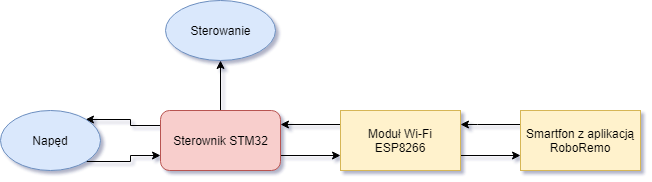
\includegraphics[width=0.8\textwidth]{figures/diagram.png}
	\caption{Architektura systemu}
	\label{fig:Architektura}
\end{figure}

%Obecne we wszystkich dokumentach
\section{Konfiguracja mikrokontrolera}

\begin{figure}[H]
	\centering
	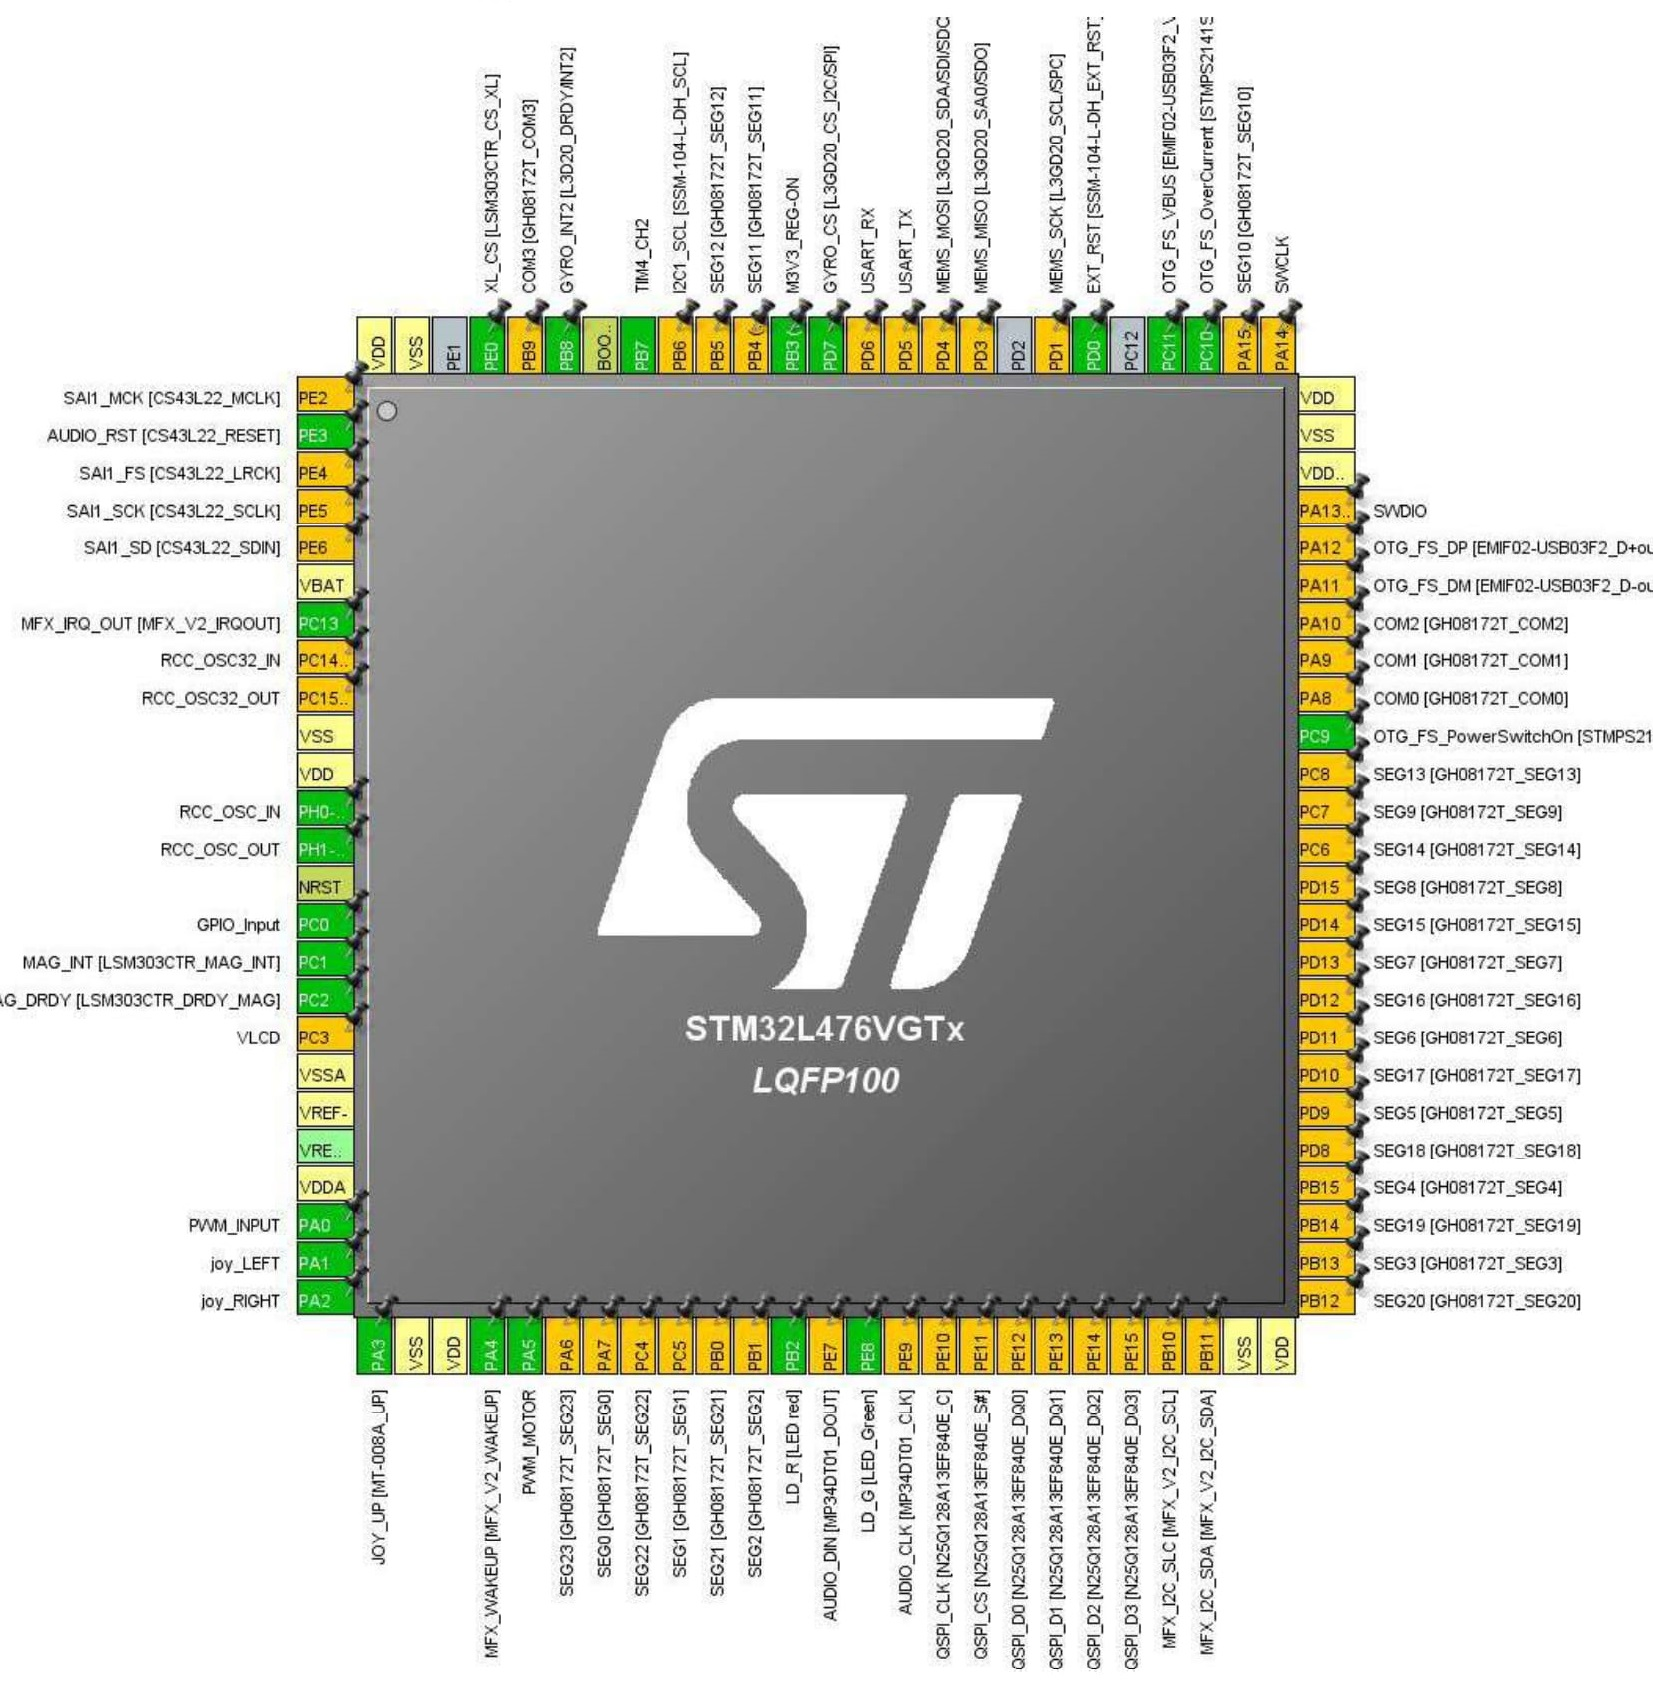
\includegraphics[width=1\textwidth]{figures/schemat-1.jpg}
	\caption{Konfiguracja wyjść mikrokontrolera w programie STM32CubeMX}
	\label{fig:KonfiguracjaMikrokontrolera}
\end{figure}

\newpage
\begin{figure}[H]
	\centering
	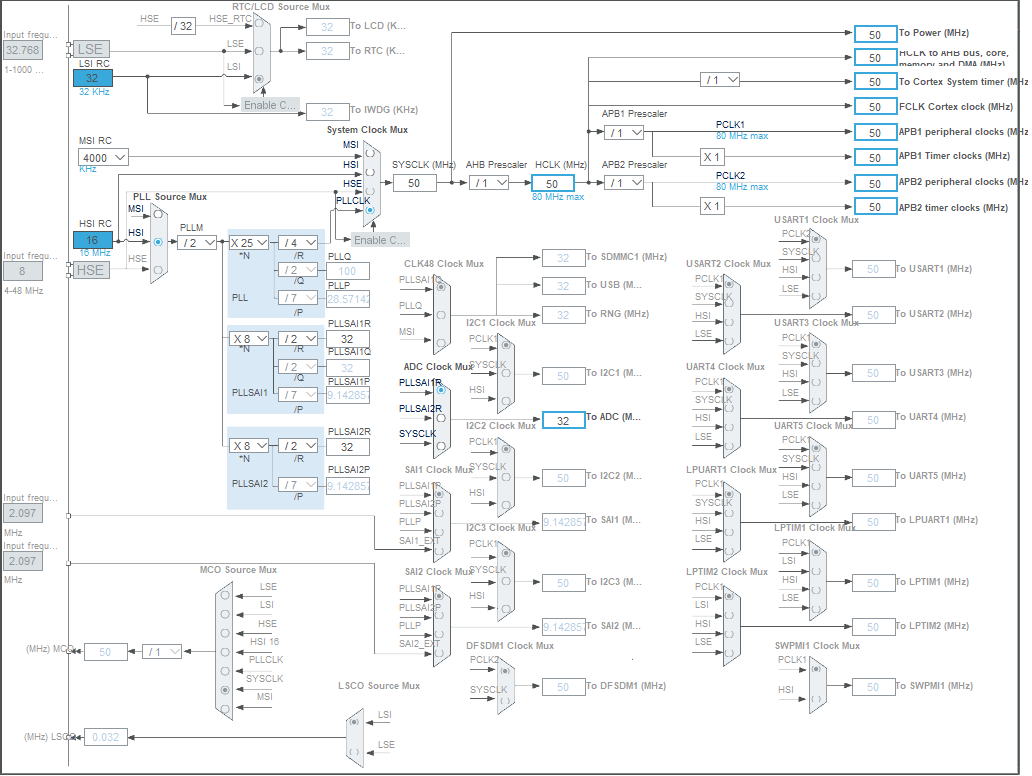
\includegraphics[width=0.9\textheight,angle=90]{figures/zegar.png}
	\caption{Konfiguracja zegarów mikrokontrolera}
	\label{fig:KonfiguracjaZegara}
\end{figure}

%Obecne we wszystkich dokumentach
\subsection{Konfiguracja pinów}

\begin{table}[H]
	\centering
	\begin{tabular}{|l|l|l|l|}
		\hline
		PIN & Tryb pracy & Funkcja/etykieta\\
		\hline
		PC14 & OSC32\_IN*	RCC\_OSC32\_IN	&\\
		PC15 & OSC32\_OUT*	RCC\_OSC32\_OUT	&\\
		PH0&  OSC\_IN*	RCC\_OSC\_IN	&\\
		PH1&  OSC\_OUT*&		RCC\_OSC\_OUT	\\
		PA2&	USART2\_TX&	USART\_TX\\
		PA3&	USART2\_RX&	USART\_RX\\
		%PE11&	TIM1\_CH2&	PWM\_SERVO\\
		PA0& TIM5\ CH1& ENCODER\_P \\
		PA5&	TIM2\_CH1&	DO\_PRZODU\\
		PB6&    TIM4\_CH1&	SERVO\\
		
		
		\hline
	\end{tabular}
	\caption{Konfiguracja pinów mikrokontrolera}
\end{table}

%Obecne we wszystkich dokumentach
\subsection{USART}

Interfejs jest wykorzystywany do komunikacji z modułem Wi-Fi (ESP8266). Moduł odbiera dane za pomocą interfejsu UDP i przekazuje je do mikrokontrolera STM32 za pomocą interfejsu komunikacji szeregowej.

\begin{table}[H]
	\centering
	\begin{tabular}{|l|c|} \hline
		\textbf{Parametr} & Wartość \\
		\hline
		\hline  \textbf{Baud Rate}&115200  \\\hline
		\textbf{Word Length } & \textcolor{blue}{8 Bits (including parity)}\\\hline
		\textbf{Parity} &  None\\
		\hline
		\textbf{Stop Bits}& 1\\
		\hline
	\end{tabular}
	\caption{Konfiguracja peryferium USART}
	\label{tab:USART}
\end{table}

\subsection{Timer 2}

\begin{table}[H]
	\centering
	\begin{tabular}{|l|c|} \hline
		\textbf{Parametr} & Wartość \\
		\hline
		\hline  \textbf{Clock Source}&Internal Clock  \\\hline
		\textbf{Channel1} & PWM Generation CH1\\\hline
		\textbf{Prescaler} & \textcolor{blue}{TIM2\_PRESC}\\\hline
		\textbf{Counter Mode} &  Up\\
		\hline
		\textbf{Counter Period}& \textcolor{blue}{TIM2\_PERIOD}\\\hline
		\textbf{Internal Clock Division}& No Division\\
		\hline
		\textbf{Mode}& PWM mode 1\\
		\hline
		\textbf{CH Polarity}& High\\
		\hline
	\end{tabular}
	\caption{Konfiguracja peryferium Timer 2}
	\label{tab:Timer2}
\end{table}

\subsection{Timer 4}

\begin{table}[H]
	\centering
	\begin{tabular}{|l|c|} \hline
		\textbf{Parametr} & Wartość \\
		\hline
		\hline  \textbf{Clock Source}&Internal Clock  \\\hline
		\textbf{Channel} & PWM Generation CH1\\\hline
		\textbf{Prescaler} & \textcolor{blue}{TIM4\_PRESC}\\\hline
		\textbf{Counter Mode} &  Up\\
		\hline
		\textbf{Counter Period}& \textcolor{blue}{TIM4\_PERIOD}\\\hline
		\textbf{Internal Clock Division}& No Division\\
		\hline
		\textbf{Mode}& PWM mode 1\\
		\hline
		\textbf{CH Polarity}& High\\
		\hline
	\end{tabular}
	\caption{Konfiguracja peryferium Timer 4}
	\label{tab:Timer4}
\end{table}

\subsection{Timer 5}

\begin{table}[H]
	\centering
	\begin{tabular}{|l|c|} \hline
		\textbf{Parametr} & Wartość \\
		\hline
		\hline  \textbf{Clock Source}&Internal Clock  \\\hline
		\textbf{Channel} & Input Capture direct mode\\\hline
		\textbf{Prescaler} & \textcolor{blue}{TIM5\_PRESC}\\\hline
		\textbf{Counter Mode} &  Up\\
		\hline
		\textbf{Counter Period}& \textcolor{blue}{TIM5\_PERIOD}\\\hline
		\textbf{Internal Clock Division}& No Division\\
		\hline
	\end{tabular}
	\caption{Konfiguracja peryferium Timer 6}
	\label{tab:Timer6}
\end{table}
%Obecne w dokumencie do etapu II oraz III
\section{Urządzenia zewnętrzne}
	\subsection{Moduł Wi-Fi ESP8266}
	Moduł dobiera dane za pomocą protokołu UDP i przekazuje je odpowiednio sformatowane za pomocą portu szeregowego do mikrokontrolera STM32. Do oprogramowania modułu wykorzystano framework Arduino. \\
	Ustawienia komunikacji szeregowej:
		\begin{table}[H]
			\centering
			\begin{tabular}{|l|c|} \hline
				\textbf{Parametr} & Wartość \\
				\hline
				\hline  \textbf{Baud Rate}&115200  \\\hline
				\textbf{Word Length } & 8 Bits (including parity)\\\hline
				\textbf{Parity} &  None\\
				\hline
				\textbf{Stop Bits}& 1\\
				\hline
			\end{tabular}
			\caption{Konfiguracja peryferium UART w module Wi-Fi}
			\label{tab:UARTWiFI}
		\end{table}
	
	\subsection{Smartfon z aplikacją RoboRemo}
	Przesyła wartości osi X i Y żyroskopu za pomocą protokołu UDP. \\ 
	Ustawienia żyroskopu w aplikacji:
	\begin{table}[H]
		\centering
		\begin{tabular}{|l|c|} 
			\hline
			\textbf{Parametr} & Wartość \\
			\hline
			\hline  \textbf{Etykieta}&x  \\\hline
			 \textbf{Wzmocnienie}&1.0  \\\hline
			\textbf{Typ danych} & int\\\hline
			\textbf{Zakres} &  od -255 do 255\\
			\hline
			\textbf{Limit do [min:max]}& tak\\
			\hline
		\end{tabular}
		\caption{Konfiguracja osi X}
		\label{tab:OsX}
	\end{table}

	\begin{table}[H]
		\centering
		\begin{tabular}{|l|c|} 
			\hline
			\textbf{Parametr} & Wartość \\
			\hline
			 \textbf{Etykieta}&y  \\\hline
			\hline  \textbf{Wzmocnienie}&0.5  \\\hline
			\textbf{Typ danych} & int\\\hline
			\textbf{Zakres} &  od 50 do 150\\
			\hline
			\textbf{Limit do [min:max]}& tak\\
			\hline
		\end{tabular}
		\caption{Konfiguracja osi Y}
		\label{tab:OsY}
	\end{table}

%Obecne w dokumencie do etapu II oraz III
\section{Projekt elektroniki}
	\subsection{Połączenie pomiędzy STM32 a modułem WiFi}
		\begin{figure}[H]
			\centering
			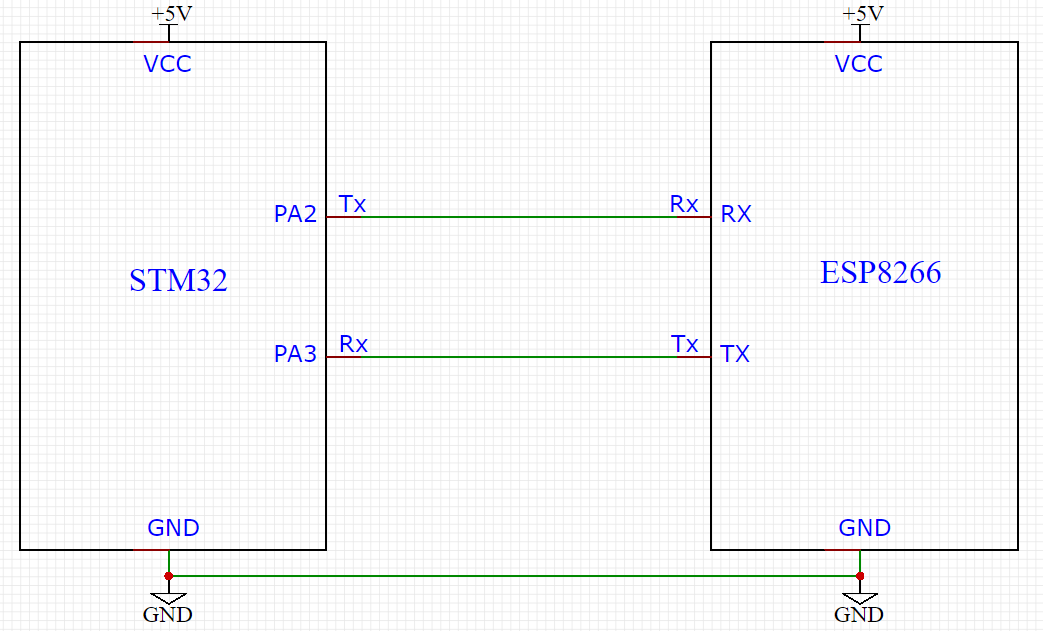
\includegraphics[width=0.8\textwidth]{figures/uart.png}
			\caption{Połączenie STM32 z ESP8266}
			\label{fig:UART}
		\end{figure}
	
	\subsection{Schemat połączenia z serwomechanizmem}
	\begin{figure}[H]
		\centering
		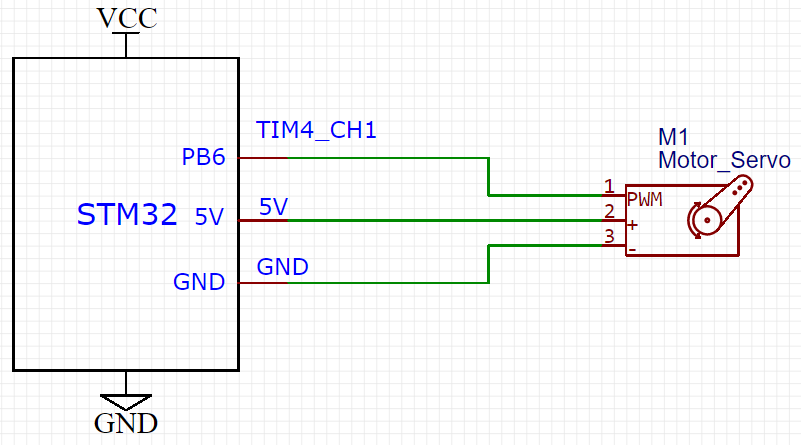
\includegraphics[width=0.8\textwidth]{figures/servo.png}
		\caption{Połączenie STM32 z serwomechanizmem}
		\label{fig:Servo}
	\end{figure}
	
	\subsection{Schemat połączenia z silnikiem}	
	\begin{figure}[H]
		\centering
		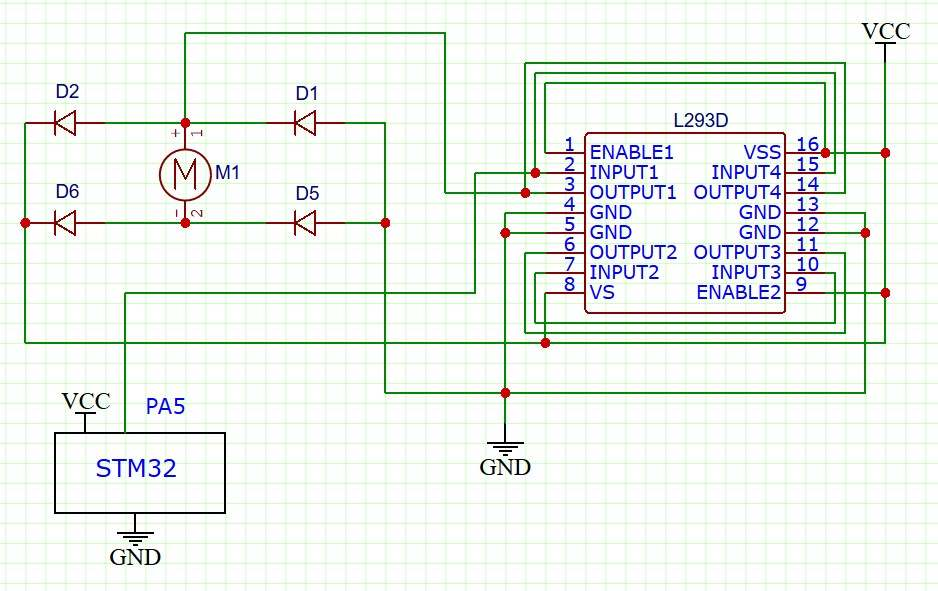
\includegraphics[width=0.8\textwidth]{figures/silnik.jpg}
		\caption{Schemat regulacji prędkości obrotowej silnika}
		\label{fig:KonfiguracjaPWM}
	\end{figure}
	
	\subsection{Schemat połączenia z enkoderem}
	\begin{figure}[H]
		\centering
		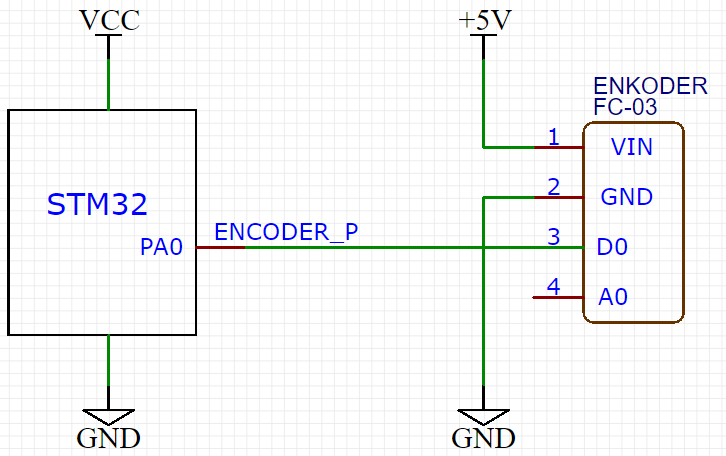
\includegraphics[width=0.8\textwidth]{figures/enkoder.png}
		\caption{Schemat połączenia mikrokontrolera z enkoderem}
		\label{fig:Enkoder}
	\end{figure}
%Obecne w dokumencie do etapu II oraz III
\section{Konstrukcja mechaniczna}

	\begin{figure}[H]
		\centering
		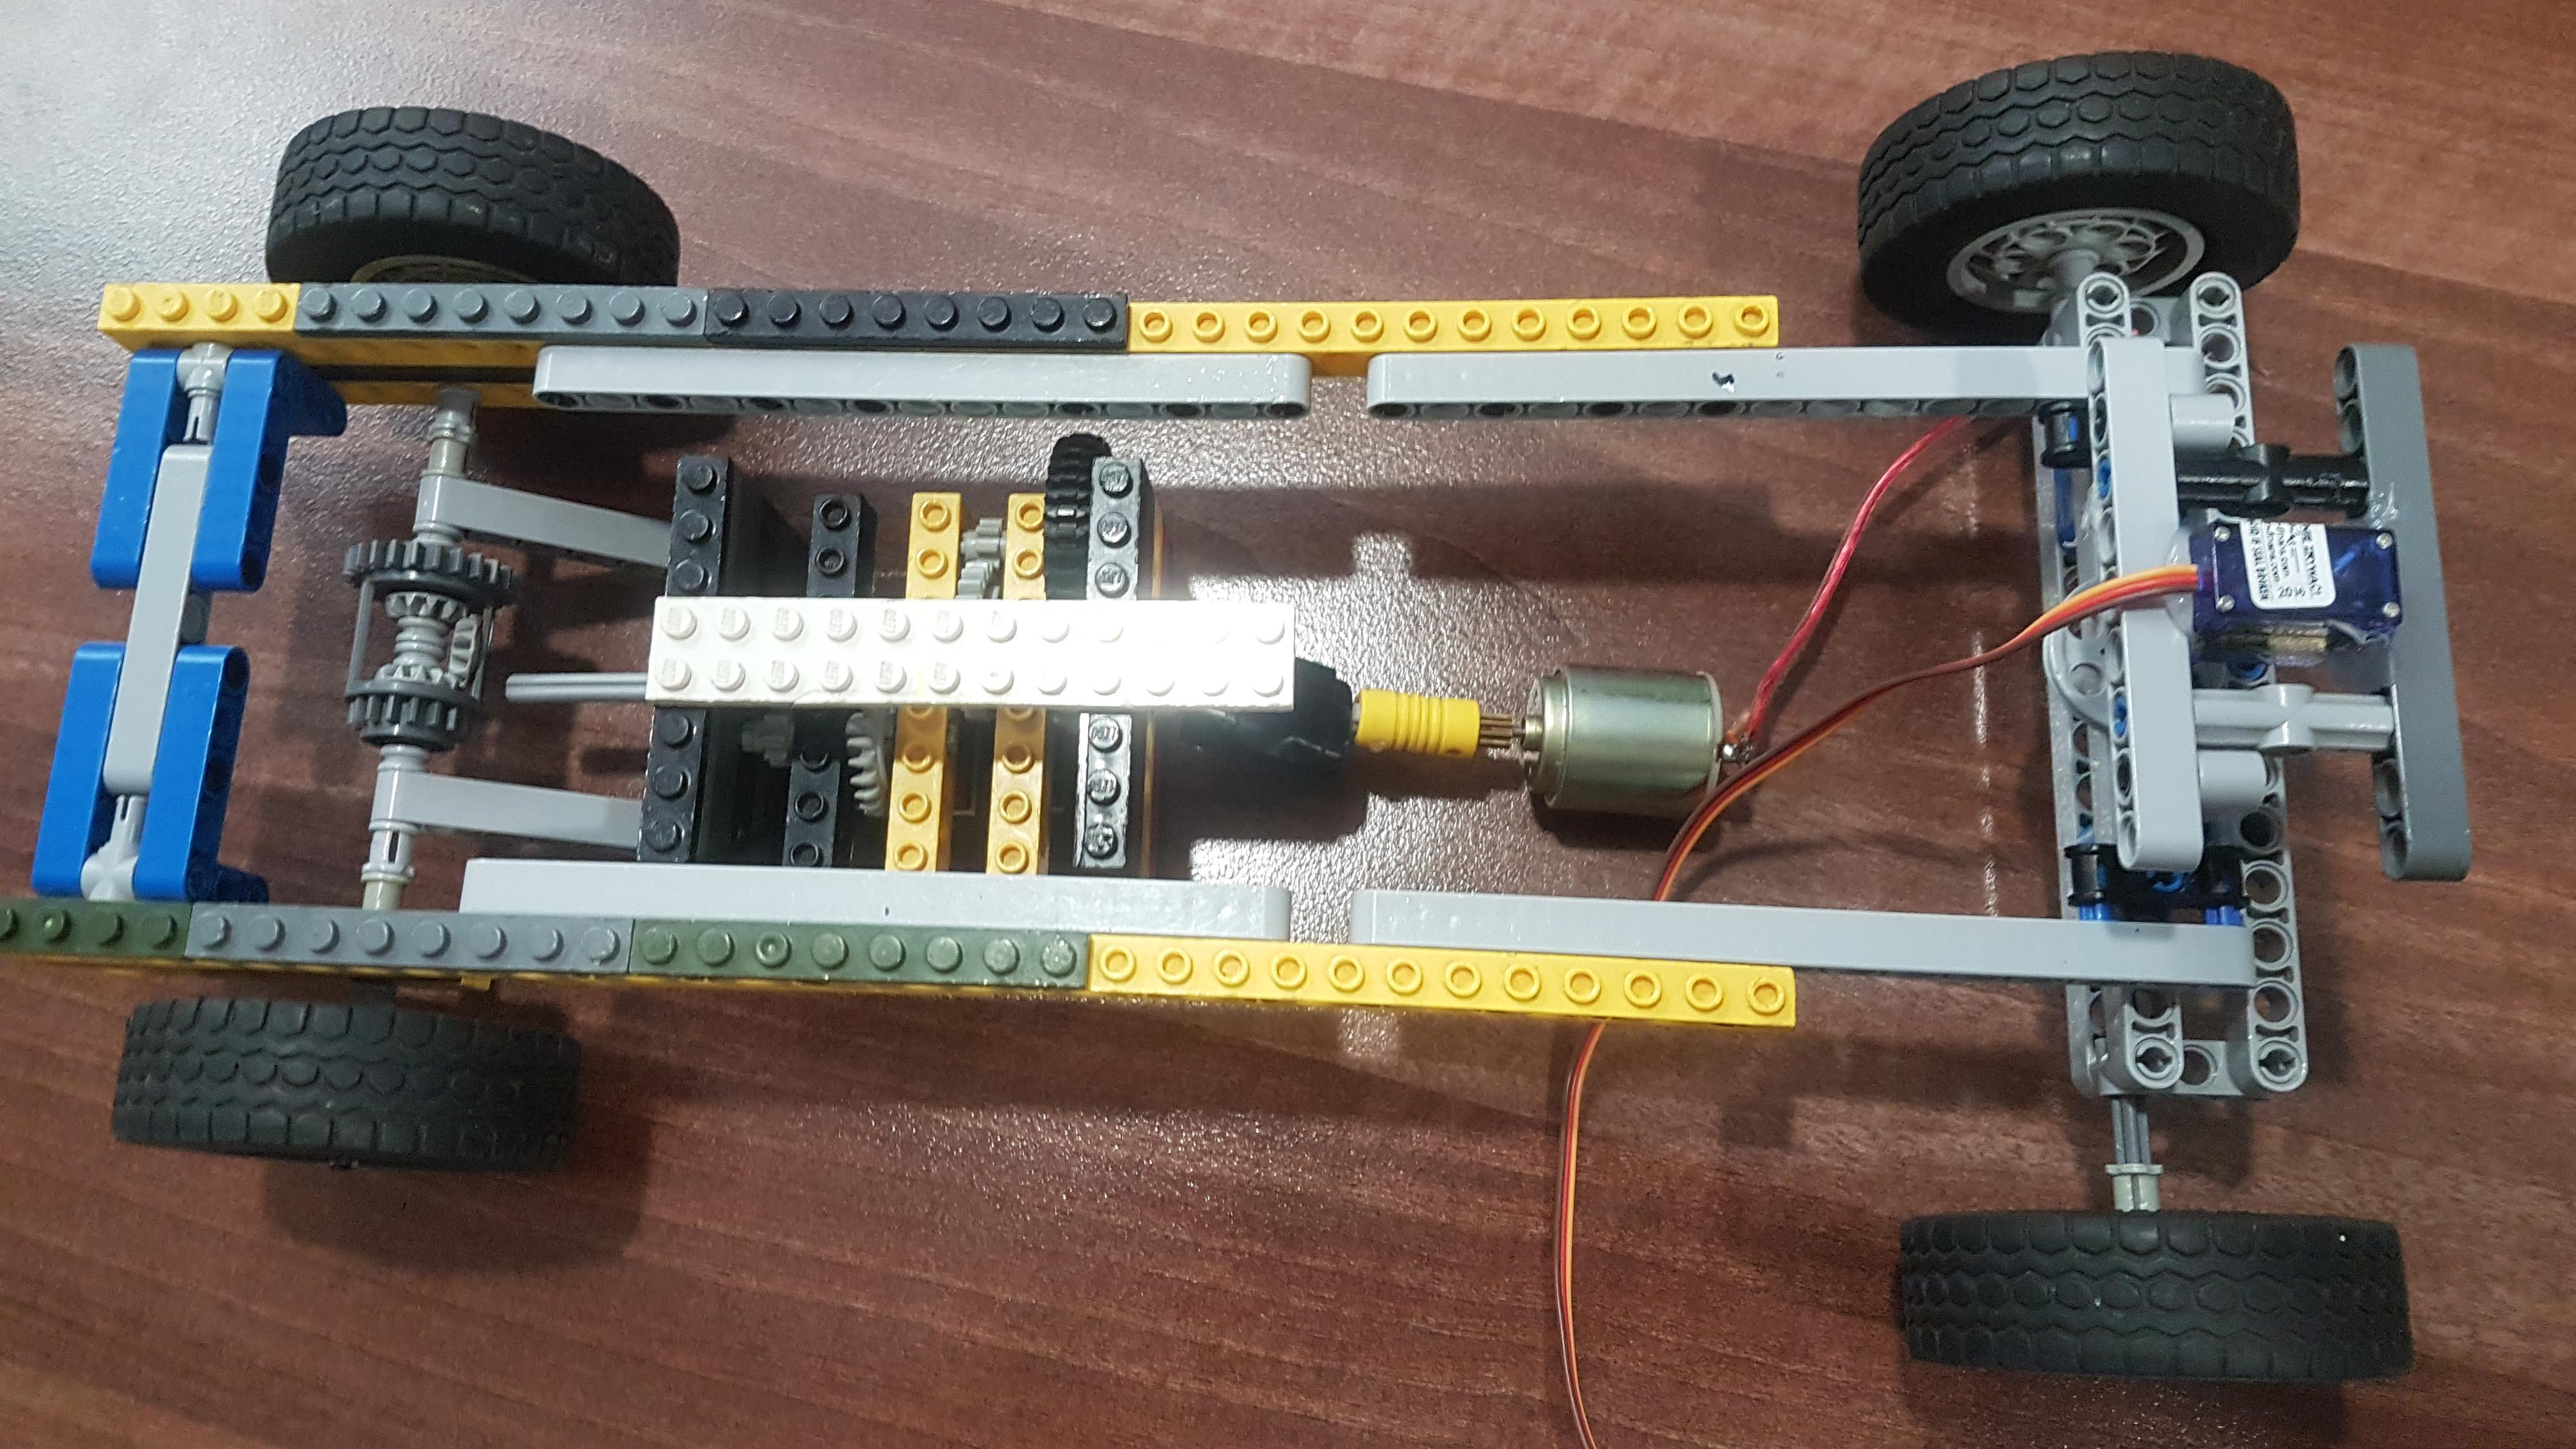
\includegraphics[width=1\textwidth]{figures/20190410_135905.jpg}
		\caption{Zdjęcie części mechanicznej}
		\label{fig:Zdjęcie części mechanicznej}
	\end{figure}
	
		\begin{figure}[H]
		\centering
		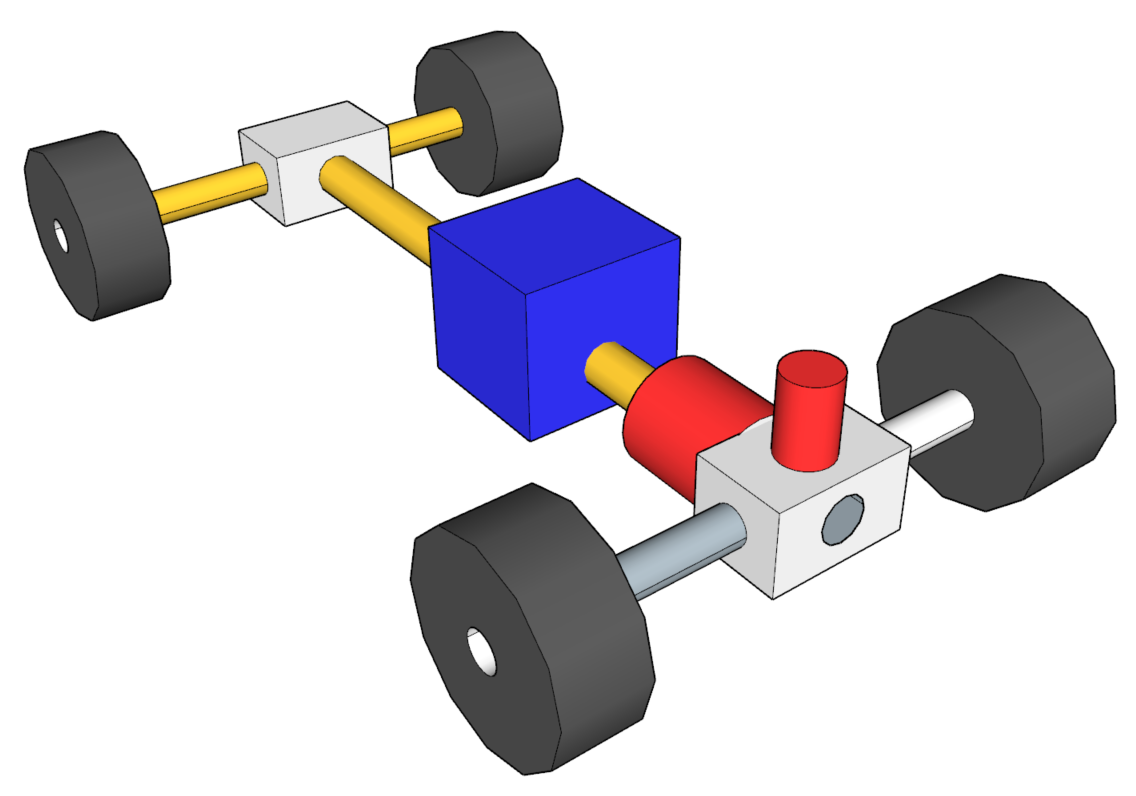
\includegraphics[width=1\textwidth]{figures/1.png}
		\caption{Schemat mechaniczny 1/2}
		\label{fig:Schemat mechaniczny 1}
	\end{figure}
	
		\begin{figure}[H]
		\centering
		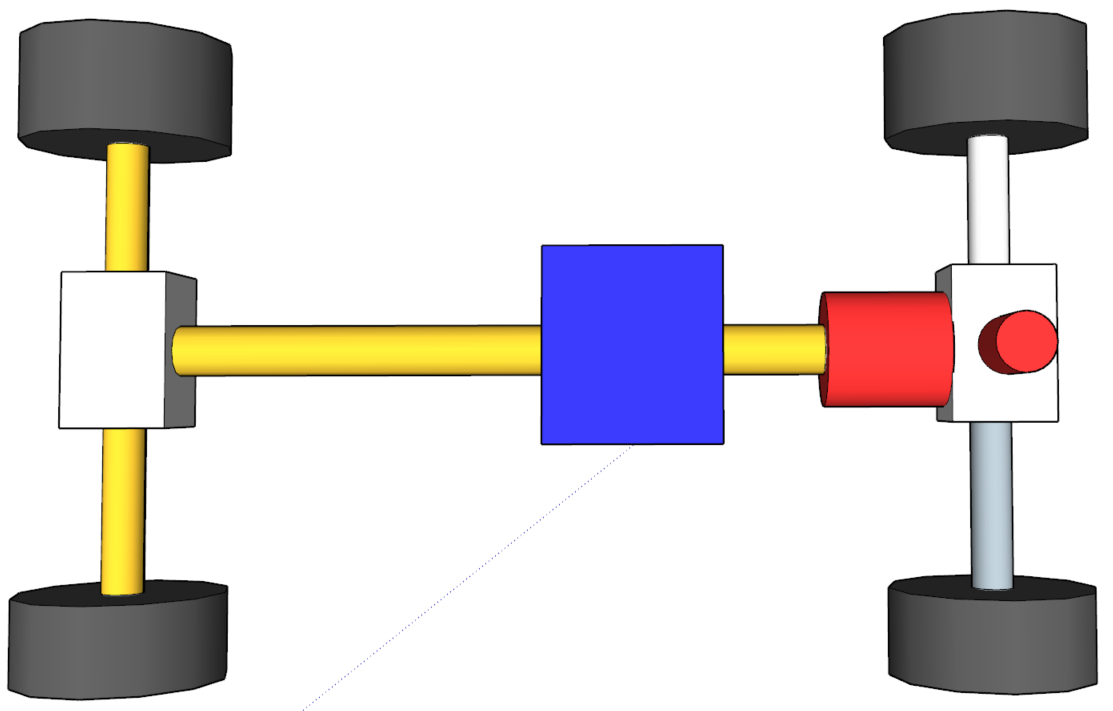
\includegraphics[width=1\textwidth]{figures/2.png}
		\caption{Schemat mechaniczny 2/2}
		\label{fig:Schemat mechaniczny 2}
	\end{figure}
	
	
		\begin{table}[H]
			\centering
			\begin{tabular}{|l|c|} \hline
				\textbf{Kolor} & \textbf{Opis} \\
				\hline  Czerwony & Silniki  \\\hline
				Niebieski & Przekładnia\\\hline
				Żółty &  Elementy przeniesienia napędu\\
				\hline
			\end{tabular}
			\caption{Legenda}
			\label{tab:Legenda}
		\end{table}

\section{Regulator PID}

\subsection{Wykres odpowiedzi skokowej}
\begin{figure}[H]
		\centering
		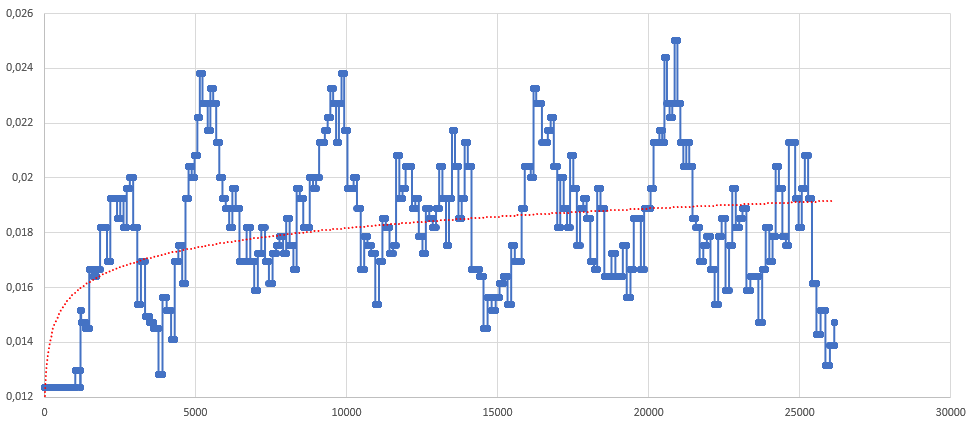
\includegraphics[width=1\textwidth]{figures/odp.png}
		\caption{Odpowiedz skokowa}
		\label{fig:Odpowiedz skokowa}
	\end{figure}
	
	Na wykresie występują bardzo duże oscylacje, które są spowodowane niedoskonałością wykonanego mechanizmu różnicowego oraz zbyt małą rozdzielczością odczytów z enkoderów. W związku z tym odpowiedź skokową przybliżono linią trendu i na jej podstawie za pomocą II metody Zieglera - Nicholsa wyliczono parametry K_{p}, K_{i} \hspace{0.1cm} oraz \hspace{0.1cm} K_{d}.
	
\subsection{Wyznaczenie parametrów PID}

\hspace{-0.55cm} k = \Delta wy / \Delta we = \frac {0.01923}{0.01515} \ = 1.2693 \approx 1.27 \newline

\hspace{-0.55cm} K_{p} = 0.6 \ast k \ = 0.762 \newline
K_{i} = 2 \ast \frac{K_{p}}{P_{u}} \ = 1.879 \newline
K_{d} = \frac{K_{p}\ast P_{u}}{8} \ = 0.086 \newline

%Obecne w dokumencie do etapu II oraz III
\section{Opis działania programu}

\subsection{Schemat działania programu}
	\begin{figure}[H]
		\centering
		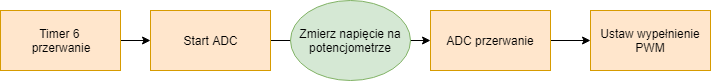
\includegraphics[width=0.8\textwidth]{figures/diagramPWM.png}
		\caption{Schemat działania programu}
		\label{fig:diagramPWM}
	\end{figure}

\subsection{Ręczna inicjalizacja parametrów w funkcji main}
	\begin{lstlisting}[tabsize=2]
	flag1 = flag2 = 0;
	pwm_dutyL = pwm_dutyP = 0;
	HAL_TIM_IC_Start_IT(&htim5, TIM_CHANNEL_1);
	HAL_TIM_IC_Start_IT(&htim5, TIM_CHANNEL_2);
	
	HAL_TIM_PWM_Start(&htim4, TIM_CHANNEL_1);
	HAL_TIM_PWM_Start(&htim2, TIM_CHANNEL_1);
	HAL_TIM_PWM_Start(&htim2, TIM_CHANNEL_2);
	
	HAL_UART_Receive_DMA(&huart2, &Received, BUFSIZE);
	PIDInit(&pid, kp, ki, kd, sampleTimeSeconds, minOutput, maxOutput, mode, control);
	PIDSetpointSet(&pid, set_value);
	PIDInputSet(&pid, speed);
	\end{lstlisting}

\subsection{Funkcja obsługująca Input Capture}
	\begin{lstlisting}[tabsize=2]
	int speed;
	void HAL_TIM_IC_CaptureCallback(TIM_HandleTypeDef *htim)
	{
		if (htim == &htim5)
		{
			if (htim->Channel == HAL_TIM_ACTIVE_CHANNEL_1)
			{
				period1 = __HAL_TIM_GET_COMPARE(&htim5, TIM_CHANNEL_1);
				__HAL_TIM_SET_COUNTER(&htim5, 0);
				flag1 = 1;
				speed = (period1 <= 50) ? (255 - map(period1, 20, 50, 0, 255)) : 0;
			}
			sampleTimeSeconds = period1 / 1000.0;
			PIDInit(&pid, kp, ki, kd, sampleTimeSeconds, minOutput, maxOutput, mode, control);
		}
	}
	\end{lstlisting}

\subsection{Funkcja obsługująca przerwanie USART}

	\begin{lstlisting}[tabsize=2]
	volatile uint8_t xvalue, yvalue, yprevious, xprevious;
	volatile char xsign;
	void HAL_UART_RxCpltCallback(UART_HandleTypeDef *huart) 
	{
		axis = (char)(Received[nrAxis]);
		sign = (char)(Received[nrSign]);
		value = (uint8_t)(Received[nrValue]);
		
		if(axis == 'x')
		{
			xsign = sign;
			xprevious = xvalue;
			xvalue = value;
		}
		
		if(axis == 'y')
		{
			yprevious = yvalue;
			yvalue = value;
			if(abs(value - xprevious) < 2)
				yvalue = yprevious;
			else if(value > 100)
				yvalue = yprevious;
			else if(value < 50)
				yvalue = yprevious;
		}
		PIDSetpointSet(&pid, set_value);
		PIDInputSet(&pid, speed);
		PIDCompute(&pid);
		pid_output = PIDOutputGet(&pid);
		HAL_UART_Receive_DMA(&huart2, &Received, BUFSIZE);
	}
	\end{lstlisting}
	
	\subsection{Funkcja realizująca jazdę}
	
	\begin{lstlisting}[tabsize=2]
	void Jazda()
	{
		__HAL_TIM_SET_COMPARE(&htim2, TIM_CHANNEL_1, 255 - pid_output);
	}
	\end{lstlisting}
	
	\subsection{Funkcja realizująca skręcanie}
	
	\begin{lstlisting}[tabsize=2]
	void Skrecanie()
	{
		__HAL_TIM_SET_COMPARE(&htim4, TIM_CHANNEL_1, yvalue);
	}
	\end{lstlisting}
	
	\subsection{Funkcja mapująca wartości czasowe na wartość zadaną regulatora PID}
	\begin{lstlisting}[tabsize=2]
	long map(long x, long in_min, long in_max, long out_min, long out_max)
	{
		return (x - in_min) * (out_max - out_min) / (in_max - in_min) + out_min;
	}
	\end{lstlisting}
	
	\subsection{Funkcja przekierowująca printf()}
	\begin{lstlisting}[tabsize=2]
	int _write(int file, char *s, int len)
	{
		HAL_UART_Transmit_DMA(&huart2, (uint8_t*)s, len);
		return len;
	}
	\end{lstlisting}
	
	\subsection{Pętla główna}
	\begin{lstlisting}[tabsize=2]
	while (1)
	{
		Jazda();
		Skrecanie();
	}
	\end{lstlisting}

%Obecne w dokumencie do etapu II oraz III (jeśli coś zostało niezrealizowane)
%\section{Zadania niezrealizowane}


%Obecne we wszystkich dokumentach
\section{Podsumowanie}
Udało się zrealizować wszystkie założenia projektowe. Jedynym elementem w projekcie, który mógłby być lepszy to kółko szczerbinkowe na osi o większej ilości dziurek, aby zwiększyć rozdzielczość odczytów z enkoderów przez co działanie regulatora PID byłoby bardziej płynne i dokładne.


\newpage
\addcontentsline{toc}{section}{Bibilografia}

\begin{thebibliography}{9}
	\bibitem{pa} Krzysztof Amborski, Andrzej Murusak:
	\emph{Teoria sterowania w ćwiczeniach}, ('78)
	
	\bibitem{pa1} Józef Lisowski:
	\emph{Podstawy automatyki}, (2015)
	
	\bibitem{pa1} Jerzy Brzózka:
	\emph{Regulatory i układy automatyki}, (2004)
	
	\bibitem{pa1} Krzysztof Tchoń:
	\emph{Manipulatory i roboty mobilne : modele, planowanie ruchu, sterowanie}, (2000)
	
	\bibitem{pa1} Stanisław Wszelak:
	\emph{Administrowanie sieciowymi protokołami komunikacyjnymi}, (2015)

\end{thebibliography}

\end{document}







































